% Chapter 5 placeholder
 %図を入れる例 (図ファイルは fig/ に配置)
 %\begin{figure}[htbp]
  % \centering
   %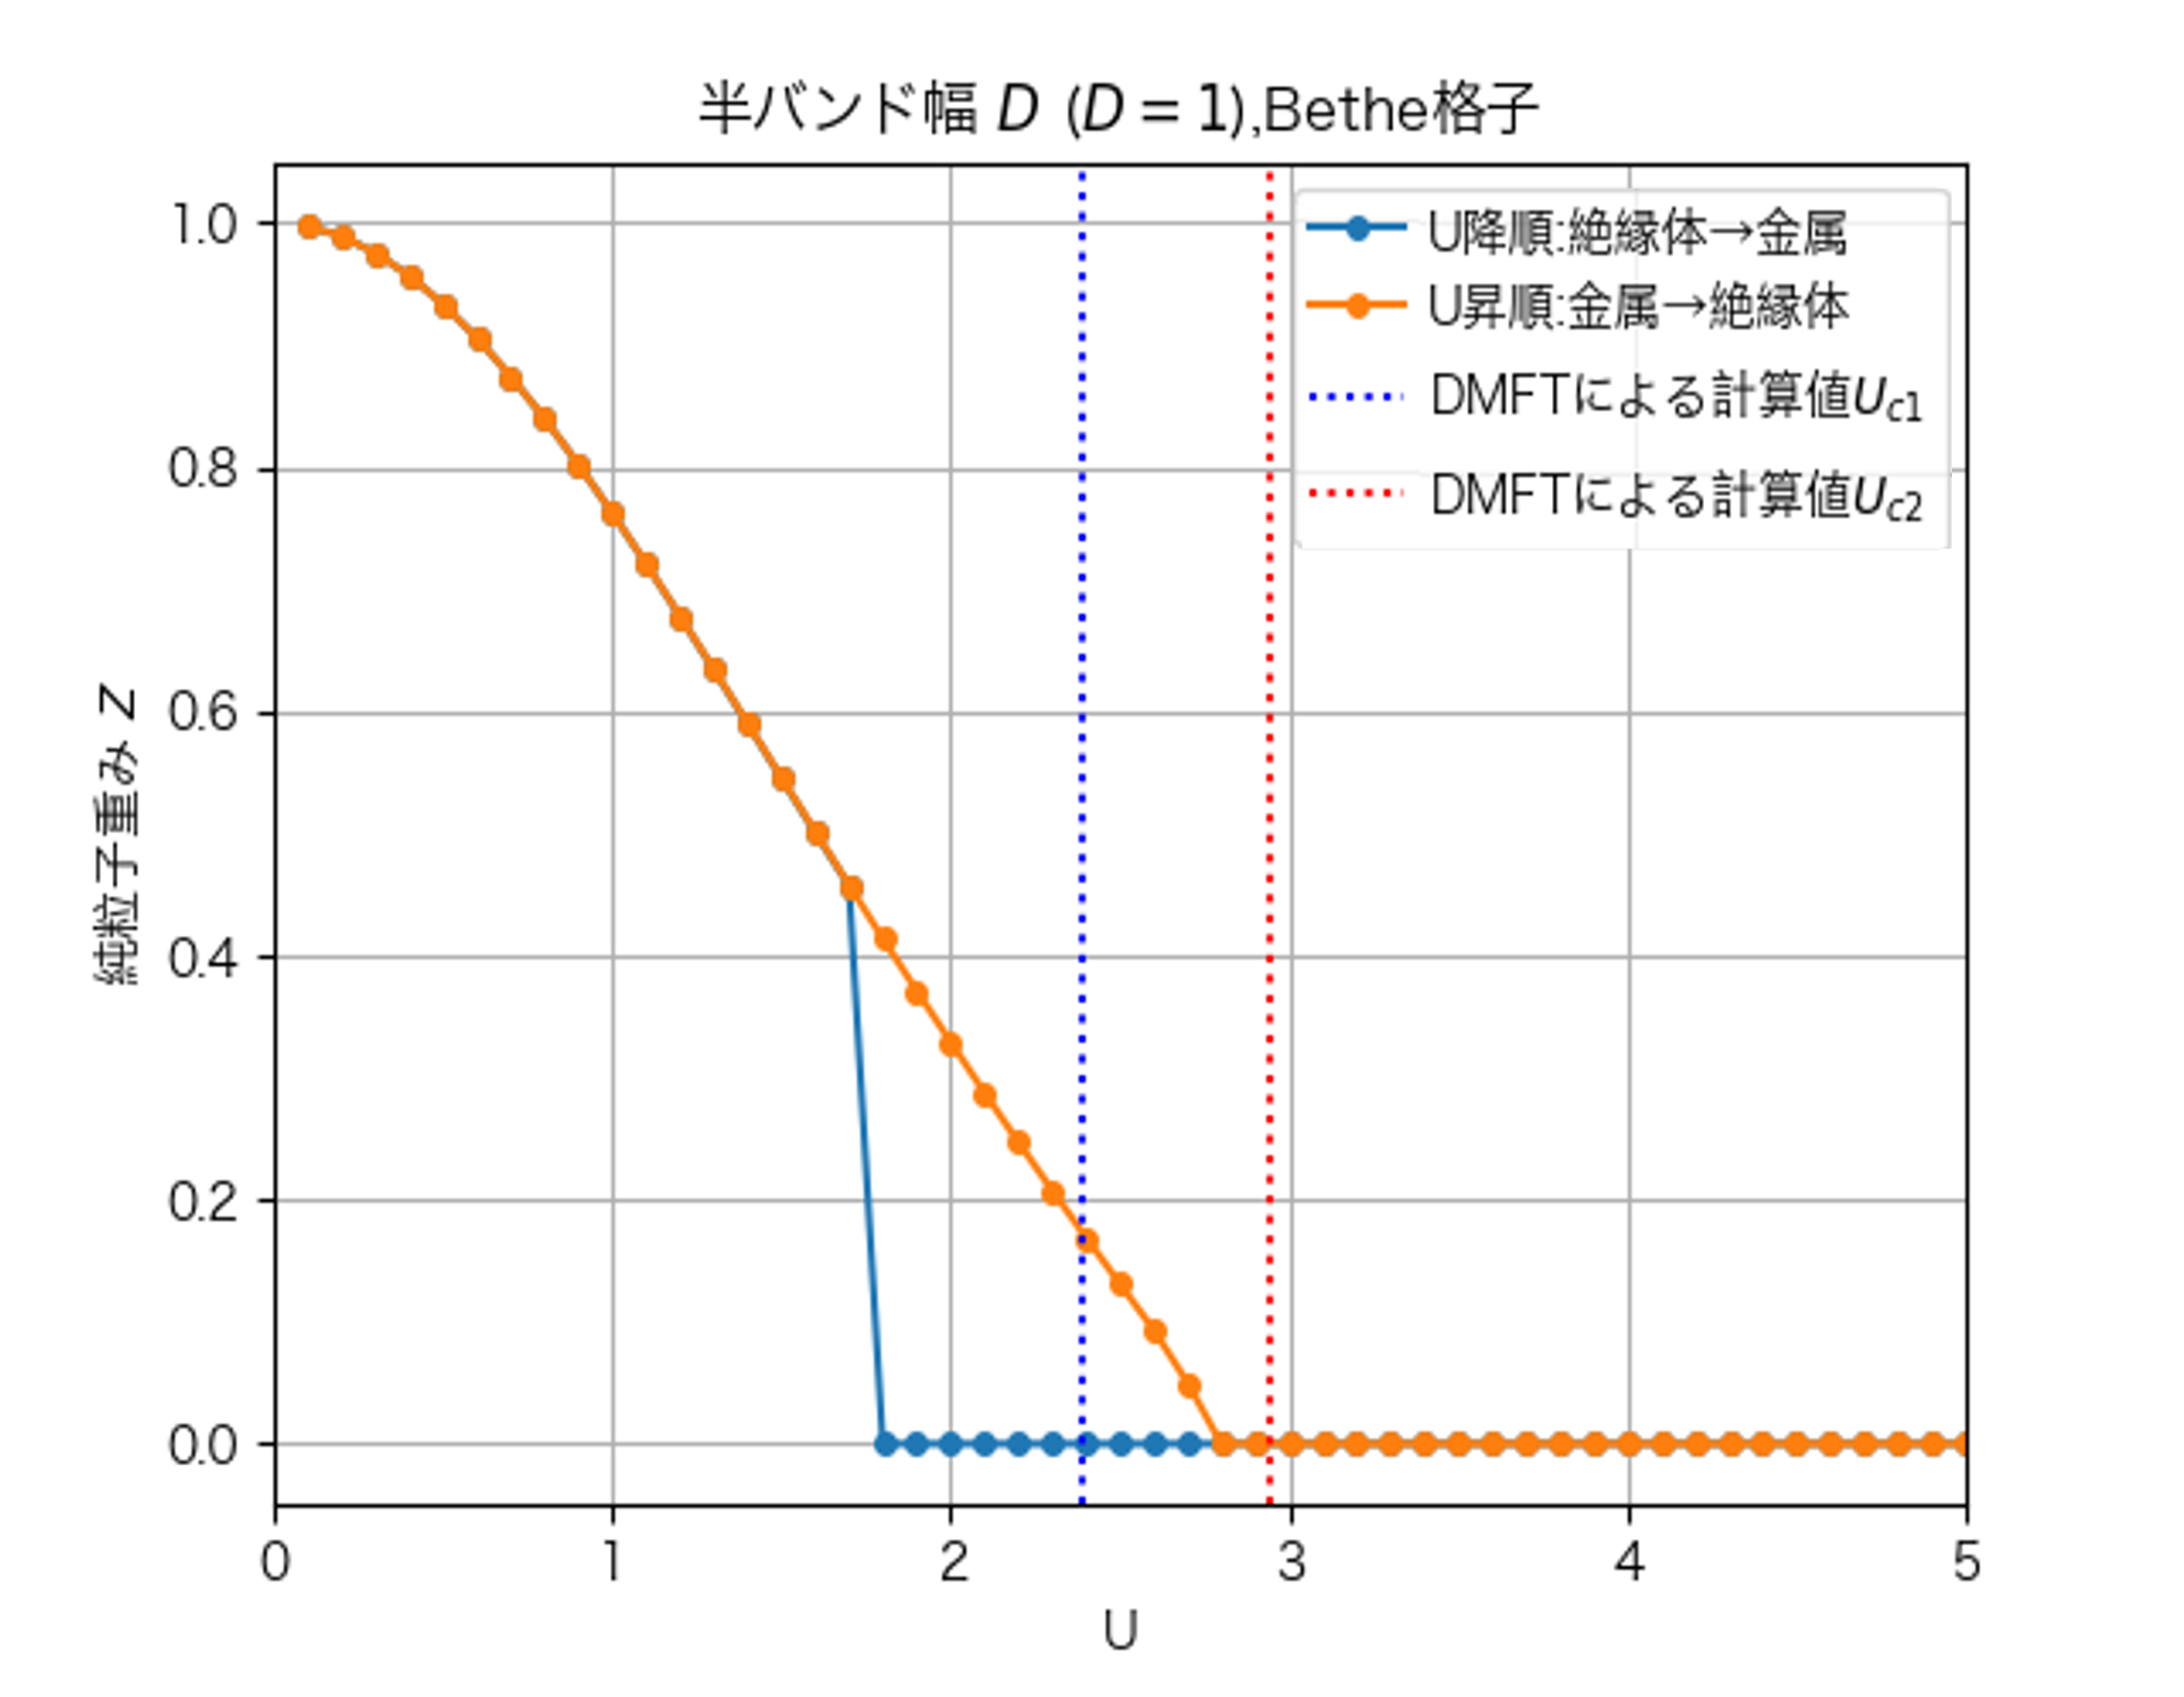
\includegraphics[width=0.9\textwidth]{fig/卒論_Bethe.png}
   %\caption{図の例}
   %\label{fig:sample}
 %\end{figure}

\section{評価指標}

本研究では金属状態とモット絶縁体状態の相転移を判定するための物理的な指標として,準粒子重み$Z$を用いた.

準粒子重み$Z$は電子が相互作用によってどれほど自由電子としての性質を失い,有効質量が増大しているかを表す量である.

$Z > 0$の有限の値を持つ場合は,系がフェルミ液体として振る舞う金属状態であることを意味する.

相互作用の増大に伴って$Z$が減少し,最終的に$Z = 0$となった状態は,電子が各サイトに完全に局在して動けなくなったモット絶縁体状態であることを意味する.

\section{結果}

前章で述べた計算条件に基づき,無限次元Bethe格子および2次元正方格子のそれぞれに対して,クーロン相互作用$U$を変化させた際の準粒子重み$Z$の振る舞いを計算した.

図\ref{fig:result_bethe}にBethe格子における計算結果を示す.

また,図\ref{fig:result_square}に2次元正方格子における計算結果を示す.

% グラフ挿入用のプレースホルダー (ファイル名をご自身の画像に書き換えてください)
 \begin{figure}[H]
     \centering
      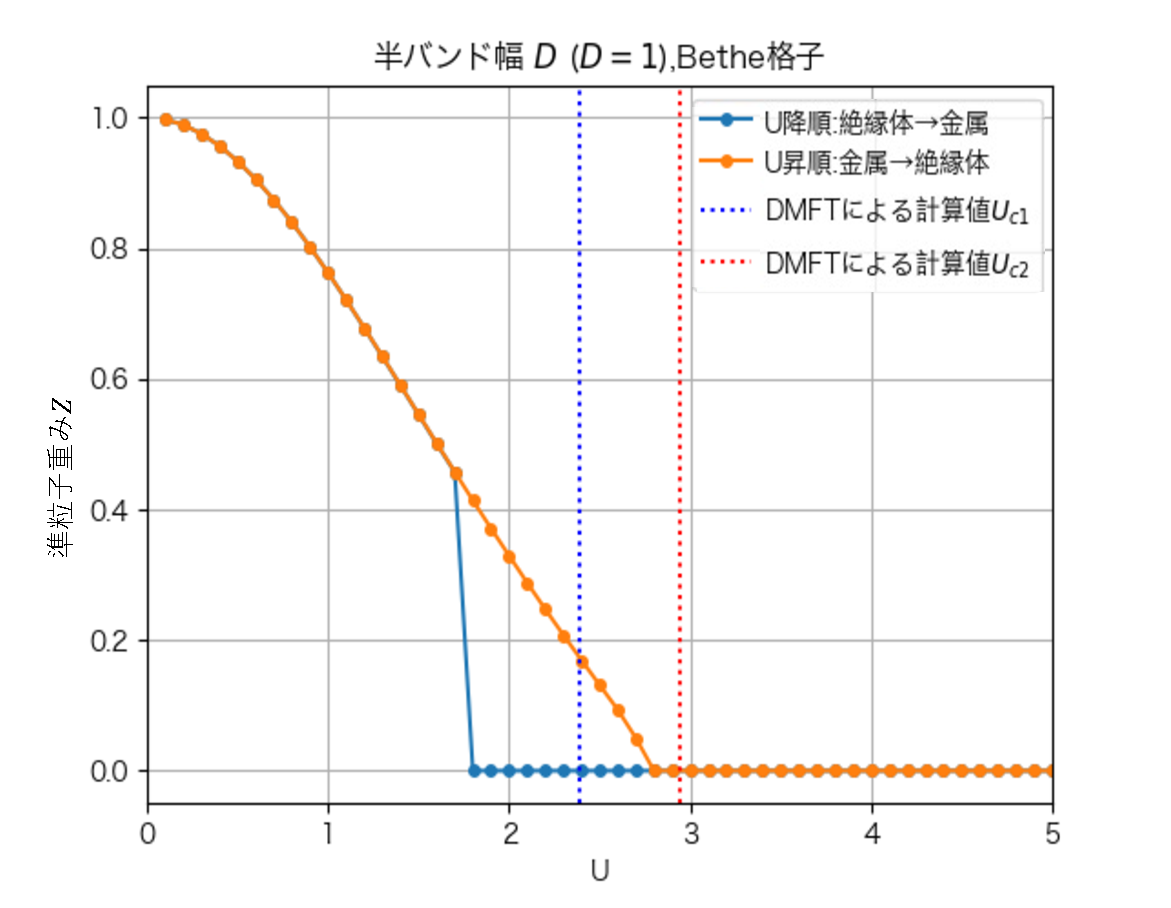
\includegraphics[width=12cm]{fig/卒論_Bethe.pdf}
          \caption{無限次元Bethe格子における準粒子重み$Z$の相互作用$U$依存性.}
    \label{fig:result_bethe}
 \end{figure}

 \begin{figure}[H]
     \centering
      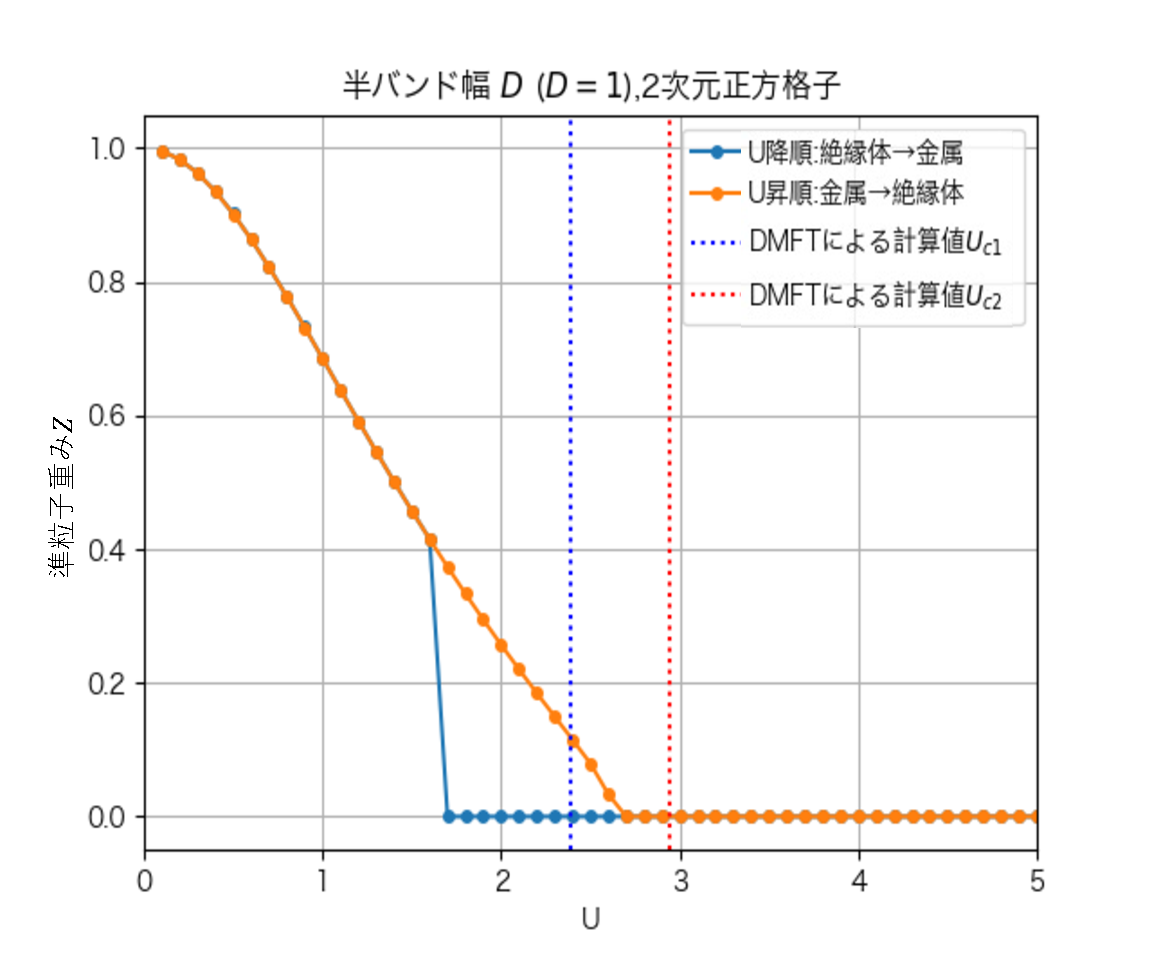
\includegraphics[width=12cm]{fig/卒論_2Dsquare.pdf}
     \caption{2次元正方格子における準粒子重み$Z$の相互作用$U$依存性.}
     \label{fig:result_square}
 \end{figure}

両方の格子モデルにおいて,相互作用$U$が小さい領域では$Z$が1に近い有限の値を取り,金属状態であることが確認できる.

$U$を増加させていくと電子相関の効果によって$Z$は単調に減少し,ある臨界値で不連続に$Z=0$へと落ち込む一次相転移の振る舞いが見られた.

さらに,金属相を初期値とする昇順スイープと,絶縁体相を初期値とする降順スイープで異なる経路をたどるヒステリシスループが明確に観測された.

このヒステリシスの存在は,金属状態の解とモット絶縁体状態の解が共存する領域があることを示している.

\section{考察}

本研究で得られた計算結果を,無限次元において厳密となる動的平均場理論による結果と比較して考察する.

動的平均場理論の計算によると,Bethe格子におけるモット転移の臨界値は,絶縁体解が消失する転移点が$U_{c1} = 2.39$,金属解が消失する転移点が$U_{c2} = 2.94$であると知られている.

図\ref{fig:result_bethe}に示された結果において,降順スイープで$Z$が立ち上がる点と,昇順スイープで$Z$が消失する点は,これらの厳密な臨界値$U_{c1}$および$U_{c2}$と極めて良い一致を見せている.

これは,補助空間を導入して変分空間を拡張したghost Gutzwiller近似が,モット転移の物理を定量的に高い精度で記述できていることを証明している.

また,次元性の影響を考察するため,Bethe格子の結果と2次元正方格子の結果を比較する.

有限次元の格子モデルである2次元正方格子においても,同様のモット転移とヒステリシスループが観測された.

最後に計算コストの観点から本手法の有用性について述べる.

動的平均場理論において連続時間量子モンテカルロ法などの厳密な不純物ソルバーを用いた場合,膨大な計算時間と並列計算リソースが必要となる.

一方,ghost Gutzwiller近似では単一の計算機を用いた極めて短い計算時間で,動的平均場理論に匹敵する高精度な結果を得ることができた.

この圧倒的な計算コストの低さは,本手法が今後より複雑な多軌道系や大規模な格子モデルへ適用可能な強力な手法であることを示唆している.